\chapter{Przypadki użycia}

\begin{usecase}
    \addfield{Akcja:}{Logowanie do aplikacji}
    \addfield{Rodzaj:}{Logowanie}
    \addfield{Aktor:}{Użytkownik}
    \addfield{Oczekiwany rezultat:}{Zalogowanie do aplikacji}

    \addscenario{Scenariusz główny:}{
    \item Użytkownik uruchamia aplikację.
    \item System wyświetla okienko logowania.
    \item Użytkownik wpisuję login i hasło.
    \item System sprawdza login i hasło użytkownika.
    \item System loguje użytkownika.
    }
    \addscenario{Scenariusz alternatywny (błędny login lub hasło):}{
    \item[1--3.] Jak w scenariuszu głównym.
    \item[4.] System wyświetla informację o błędzie, powrót do kroku 2 scenariusza głównego.
    }
\end{usecase}

\newpage
\begin{usecase}
    \addfield{Akcja:}{Wylogowanie się z aplikacji}
    \addfield{Rodzaj:}{Logowanie}
    \addfield{Aktor:}{Użytkownik}
    \addfield{Warunki:}{Zalogowany użytkownik}
    \addfield{Oczekiwany rezultat:}{Wylogowanie się z aplikacji}

    \addscenario{Scenariusz główny:}{
    \item Użytkownik klika wyloguj.
    \item System usuwa sesję użytkownika.
    \item System przekierowuje użytkownika na widok logowania.
    }
\end{usecase}

\newpage
\begin{usecase}
    \addfield{Akcja:}{Dodanie użytkownika}
    \addfield{Rodzaj:}{Zarządzanie użytkownikami}
    \addfield{Aktor:}{Administrator}
    \addfield{Warunki:}{Zalogowany użytkownik}
    \addfield{Oczekiwany rezultat:}{Dodanie do systemu nowego użytkownika}

    \addscenario{Scenariusz główny:}{
    \item Administrator klika opcję dodania nowego użytkownika.
    \item System wyświetla formatkę do wpisania loginu, hasła oraz roli nowego użytkownika.
    \item Administrator podaje dane.
    \item System tworzy nowego użytkownika.
    }
    \addscenario{Scenariusz alternatywny (zajęty login):}{
    \item[1--3.] Jak w scenariuszu głównym.
    \item[4.] System wyświetla informację o zajętym loginie, powrót do kroku 2 scenariusza głównego.
    }
\end{usecase}

\begin{usecase}
    \addfield{Akcja:}{Przeglądanie użytkowników}
    \addfield{Rodzaj:}{Zarządzanie użytkownikami}
    \addfield{Aktor:}{Administrator}
    \addfield{Warunki:}{Zalogowany użytkownik}
    \addfield{Oczekiwany rezultat:}{Wyświetlenie przez system użytkowników}

    \addscenario{Scenariusz główny:}{
    \item Administrator przegląda użytkowników.
    \item System wyświetla listę wszystkich użytkowników aplikacji wraz z ich loginami oraz hasłem.
    }
\end{usecase}

\newpage
\begin{usecase}
    \addfield{Akcja:}{Edycja użytkowników -- rozszerza przeglądanie użytkowników}
    \addfield{Rodzaj:}{Zarządzanie użytkownikami}
    \addfield{Aktor:}{Administrator}
    \addfield{Warunki:}{Zalogowany użytkownik}
    \addfield{Oczekiwany rezultat:}{Edytowanie istniejącego użytkownika}

    \addscenario{Scenariusz główny:}{
    \item Administrator wybiera z listy użytkownika, którego chce edytować.
    \item System wyświetla aktualne dane użytkownika i pozwala administratorowi edytować je.
    \item Administrator edytuje dane użytkownika.
    \item System zapisuje zmienione dane i przekierowuje administratora na listę użytkowników.
    }
    \addscenario{Scenariusz alternatywny (zajęty login):}{
    \item[1--2.] Jak w scenariuszu głównym.
    \item[3.] System wyświetla informację o zajętym loginie, powrót do kroku 2 scenariusza głównego.
    }
\end{usecase}

\begin{usecase}
    \addfield{Akcja:}{Usuwanie użytkowników -- rozszerza przeglądanie użytkowników}
    \addfield{Rodzaj:}{Zarządzanie użytkownikami}
    \addfield{Aktor:}{Administrator}
    \addfield{Warunki:}{Zalogowany użytkownik, użytkownik nie usuwa samego siebie}
    \addfield{Oczekiwany rezultat:}{Usunięcie użytkownika z systemu}

    \addscenario{Scenariusz główny:}{
    \item Administrator wybiera z listy użytkownika, którego chce usunąć.
    \item System usuwa użytkownika.
    }
\end{usecase}

\newpage
\begin{usecase}
    \addfield{Akcja:}{Dodanie pojazdu}
    \addfield{Rodzaj:}{Zarządzanie pojazdami}
    \addfield{Aktor:}{Użytkownik}
    \addfield{Warunki:}{Zalogowany użytkownik}
    \addfield{Oczekiwany rezultat:}{Dodanie nowego pojazdu do systemu}

    \addscenario{Scenariusz główny:}{
    \item Użytkownik wybiera opcję dodania pojazdu.
    \item System wyświetla formatkę zawierająca rodzaj pojazdu, numer rejestracyjny, przestrzeń ładunkową,
    rodzaj przestrzeni ładunkowej, pojemność przestrzeni ładunkowej.
    \item Użytkownik wpisuje dane pojazdu.
    \item System zapisuje nowy pojazd i przekierowuje użytkownika do listy wszystkich pojazdów.
    }
    \addscenario{Scenariusz alternatywny (zajęty numer rejestracyjny):}{
    \item[1-3.] Jak w scenariuszu głównym
    \item[4.] System wyświetla informację o zajętym numerze rejestracyjnym, powrót do kroku 2 scenariusza głównego.
    }
\end{usecase}

\begin{usecase}
    \addfield{Akcja:}{Przeglądanie pojazdów}
    \addfield{Rodzaj:}{Zarządzanie pojazdami}
    \addfield{Aktor:}{Użytkownik}
    \addfield{Warunki:}{Zalogowany użytkownik}
    \addfield{Oczekiwany rezultat:}{Wyświetlenie listy pojazdów}

    \addscenario{Scenariusz główny:}{
    \item Użytkownik przegląda pojazdy.
    \item System wyświetla wszystkie pojazdy wraz z danymi tych pojazdów.
    }
\end{usecase}

\newpage
\begin{usecase}
    \addfield{Akcja:}{Edytowanie pojazdów -- rozszerza przeglądanie pojazdów}
    \addfield{Rodzaj:}{Zarządzanie pojazdami}
    \addfield{Aktor:}{Użytkownik}
    \addfield{Warunki:}{Zalogowany użytkownik}
    \addfield{Oczekiwany rezultat:}{Edycja istniejącego pojazdu}

    \addscenario{Scenariusz główny:}{
    \item Użytkownik wybiera pojazd, który chce edytować.
    \item System wyświetla dane pojazdu i pozwala edytować je użytkownikowi.
    \item Użytkownik edytuje dane pojazdu.
    \item System zapisuje zmienione dane pojazdu.
    }
    \addscenario{Scenariusz alternatywny (zajęty numer rejestracyjny):}{
    \item[1-3.] Jak w scenariuszu głównym
    \item[4.] System wyświetla informację o zajętym numerze rejestracyjnym, powrót do kroku 2 scenariusza głównego.
    }
\end{usecase}

\begin{usecase}
    \addfield{Akcja:}{Usuwanie pojazdów -- rozszerza przeglądanie pojazdów}
    \addfield{Rodzaj:}{Zarządzanie pojazdami}
    \addfield{Aktor:}{Użytkownik}
    \addfield{Warunki:}{Zalogowany użytkownik, pojazd nie występuje w grupie pojazdów}
    \addfield{Oczekiwany rezultat:}{Usunięcie istniejącego pojazdu}

    \addscenario{Scenariusz główny:}{
    \item Użytkownik wybiera pojazd, który chce usunąć.
    \item System usuwa pojazd.
    }
\end{usecase}

\newpage
\begin{usecase}
    \addfield{Akcja:}{Łączenie pojazdów w zespoły -- rozszerza przeglądanie pojazdów}
    \addfield{Rodzaj:}{Zarządzanie pojazdami}
    \addfield{Aktor:}{Użytkownik}
    \addfield{Warunki:}{Zalogowany użytkownik}
    \addfield{Oczekiwany rezultat:}{Połączenie pojazdu w zespół}

    \addscenario{Scenariusz główny:}{
    \item Użytkownik wybiera pojazd, który chce połączyć w zespół.
    \item System wyświetla pojazdy z którymi wybrany pojazd może utworzyć zespół.
    \item Użytkownik wybiera pojazd.
    \item System tworzy zespół pojazdów.
    }
\end{usecase}

\begin{usecase}
    \addfield{Akcja:}{Usuwanie zespołów pojazdów -- rozszerza przeglądanie pojazdów}
    \addfield{Rodzaj:}{Zarządzanie pojazdami}
    \addfield{Aktor:}{Użytkownik}
    \addfield{Warunki:}{Zalogowany użytkownik, pojazd posiada zespół}
    \addfield{Oczekiwany rezultat:}{Usunięcie zespołu pojazdów}

    \addscenario{Scenariusz główny:}{
    \item Użytkownik wybiera pojazd, któremu chce usunąć zespół pojazdów.
    \item System usuwa zespół pojazdów.
    }
\end{usecase}

\newpage
\begin{usecase}
    \addfield{Akcja:}{Przeglądanie ładunków pojazdów -- rozszerza przeglądanie pojazdów}
    \addfield{Rodzaj:}{Zarządzanie ładunkami}
    \addfield{Aktor:}{Użytkownik}
    \addfield{Warunki:}{Zalogowany użytkownik, pojazd posiada przestrzeń ładunkową}
    \addfield{Oczekiwany rezultat:}{Wyświetlenie ładunków pojazdu}

    \addscenario{Scenariusz główny:}{
    \item Użytkownik wybiera pojazd, którego ładunki chce przeglądać.
    \item System wyświetla ładunki, które występują w pojeździe.
    }
\end{usecase}

\begin{usecase}
    \addfield{Akcja:}{Dodawanie ładunków do pojazdu -- rozszerza przeglądanie ładunków pojazdu}
    \addfield{Rodzaj:}{Zarządzanie ładunkami}
    \addfield{Aktor:}{Użytkownik}
    \addfield{Warunki:}{Zalogowany użytkownik}
    \addfield{Oczekiwany rezultat:}{Dodanie ładunku do pojazdu}

    \addscenario{Scenariusz główny:}{
    \item Użytkownik wybiera pojazd, któremu chce dodać ładunek.
    \item System wyświetla formatkę na której użytkownik może wpisać nazwę ładunku oraz ilość.
    \item Użytkownik wpisuje dane.
    \item System dodaje ładunek do pojazdu.
    }
    \addscenario{Scenariusz alternatywny (przekroczono maksymalną ładowność pojazdu):}{
    \item[1-3.] Jak w scenariuszu głównym
    \item[4.] System wyświetla informację o przekroczonej ładowności pojazdu, powrót do kroku 2 scenariusza głównego.
    }
\end{usecase}

\newpage
\begin{usecase}
    \addfield{Akcja:}{Usuwanie ładunków z pojazdu -- rozszerza przeglądanie ładunków pojazdu}
    \addfield{Rodzaj:}{Zarządzanie ładunkami}
    \addfield{Aktor:}{Użytkownik}
    \addfield{Warunki:}{Zalogowany użytkownik}
    \addfield{Oczekiwany rezultat:}{Usunięcie ładunku z pojazdu}

    \addscenario{Scenariusz główny:}{
    \item Użytkownik wybiera pojazd, któremu chce usunąć ładunek.
    \item System usuwa ładunek z pojazdu.
    }
\end{usecase}

\begin{usecase}
    \addfield{Akcja:}{Zapis stanu aplikacji}
    \addfield{Rodzaj:}{Zarządzanie stanem aplikacji}
    \addfield{Aktor:}{Użytkownik, Administrator}
    \addfield{Warunki:}{Zalogowany użytkownik}
    \addfield{Oczekiwany rezultat:}{Utworzenie plików ze stanem aplikacji}

    \addscenario{Scenariusz główny:}{
    \item Użytkownik wybiera opcję zapisu aplikacji do plików.
    \item System tworzy w katalogu z którego aplikacja została odpalona pliki $.csv$ zawierające pojazdy, ładunki oraz
    użytkowników.
    }
\end{usecase}

\newpage
\begin{usecase}
    \addfield{Akcja:}{Wczytanie stanu aplikacji}
    \addfield{Rodzaj:}{Zarządzanie stanem aplikacji}
    \addfield{Aktor:}{Użytkownik, Administrator}
    \addfield{Warunki:}{Zalogowany użytkownik}
    \addfield{Oczekiwany rezultat:}{Wczytanie do aplikacji danych z plików}

    \addscenario{Scenariusz główny:}{
    \item Użytkownik wybiera opcję wczytania staniu aplikacji.
    \item System szuka plików zawierających pojazdy, ładunki oraz użytkowniów w katalogu aplikacji.
    \item System odczytuje stan aplikacji z plików.
    }
    \addscenario{Scenariusz alternatywny (błąd w jednym z plików):}{
    \item[1-2.] Jak w scenariuszu głównym.
    \item System wyświetla informację o błędzie wczytywania danych z pliku i nie odczytuje stanu aplikacji z plików.
    }
\end{usecase}

\begin{figure}
    \centering
    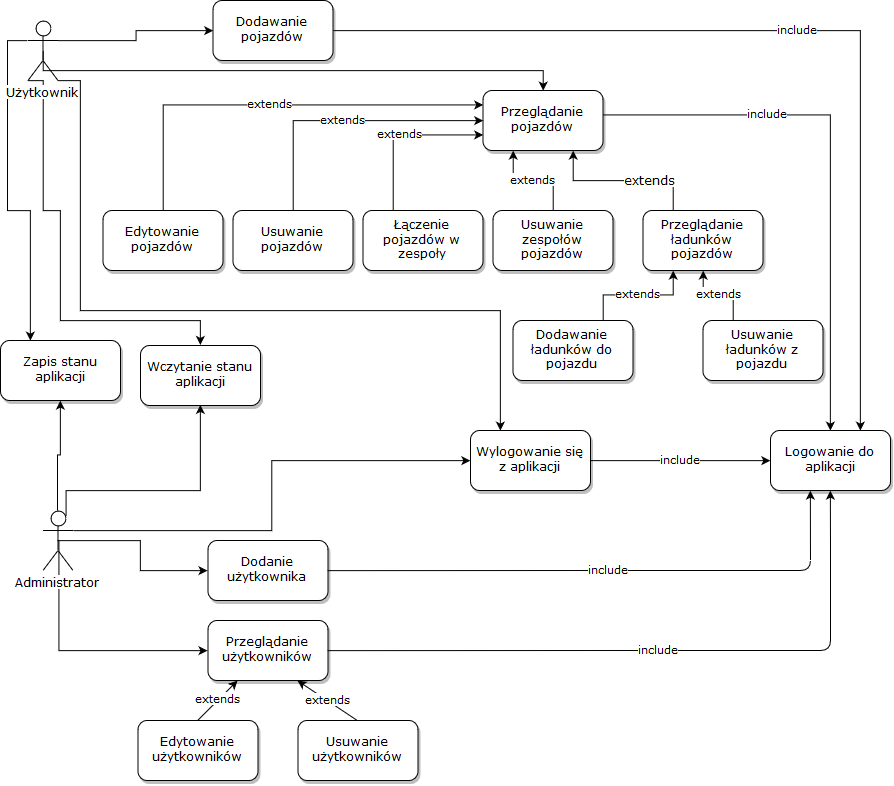
\includegraphics[width=14cm]{use-case-diagram.png}
    \caption{Diagram przypadków użycia}
\end{figure}
